\documentclass[runningheads]{llncs}
\usepackage[english]{babel}
\usepackage[utf8x]{inputenc}
\usepackage[T1]{fontenc}
\usepackage{relsize}
\usepackage{amsmath,amssymb}
\usepackage{xspace}
%% Useful packages
\usepackage{graphicx}
\usepackage{pdflscape,adjustbox}
\usepackage{multirow}

\usepackage{algorithm}
\usepackage[noend]{algpseudocode}
%\algrenewcommand{\algorithmiccomment}[1]{\hfill\texttt{//} #1}

\usepackage{booktabs} % For formal tables
\usepackage{enumitem}
\usepackage{afterpage,tabularx}
\usepackage[colorlinks=true, allcolors=blue]{hyperref}
\usepackage[square,numbers,sort]{natbib}
% Fixes for using natbib and llncs
\makeatletter
% required for natbib to have "References" printed and as section*, not chapter*
\renewcommand\bibsection%
{\section*{\refname\@mkboth{\MakeUppercase{\refname}}{\MakeUppercase{\refname}}}}
\renewcommand\@biblabel[1]{#1.}
\def\bibfont{\small}
\makeatother

% If you use the hyperref package, please uncomment the following line
% to display URLs in blue roman font according to Springer's eBook style:
\renewcommand\UrlFont{\color{blue}\rmfamily}

\newcommand{\true}{\textsc{true}}
\newcommand{\false}{\textsc{false}}
\newcommand{\NULL}{\textsc{null}}
\newcommand{\NA}{---}
\newcommand{\assign}{\ensuremath{:=}}
\newcommand{\procedure}[1]{\textsf{#1}}
\newcommand{\Inf}{\ensuremath{\infty}}
\DeclareMathOperator*{\argmax}{arg\,max}


\newcommand{\Prob}{\ensuremath{p}}
\newcommand{\minit}{\ensuremath{m_\text{ini}}\xspace}
%\newcommand{\FEmax}{\ensuremath{\textit{FE}_{\max}}}
\newcommand{\FEmax}{\ensuremath{m}}

%% Revision documents
\usepackage[dvipsnames]{xcolor}
\usepackage[normalem]{ulem}
% FIXME: \sout is not very good. It cannot handle commands within its argument.
\newcommand{\SuggestEdit}[3][red]{\textcolor{#1}{\sout{#2}}\textcolor{#1}{#3}}
\let\svthefootnote\thefootnote
\newcommand\colorfootnote[2][black]{\def\thefootnote{\color{#1}\svthefootnote}%
  \footnote{\color{#1}#2}\def\thefootnote{\color{black}\svthefootnote}}
\newcommand\RevComment[3][red]{\protect\colorfootnote[#1]{{\textbf{[#2: #3]}}}}
% Command for edits, command for commenting and color
\newcommand\newrevisor[3]{%%
  \colorlet{#1}{#3}
  \expandafter\newcommand\csname#1\endcsname[2]{\SuggestEdit[#1]{##1}{##2}}%%
  \expandafter\newcommand\csname#2\endcsname[1]{\RevComment[#1]{#2}{##1}}%%
}
\newrevisor{manuel}{MANUEL}{Purple}
\newrevisor{ekhine}{EKHINE}{red}

\hyphenation{%%% Merriam-Webster
  di-men-sion-al %%
  op-tical net-works semi-conduc-tor %%
  pher-o-mone non-dom-i-nance %%
  non-dom-i-nat-ed chro-mo-some %%
  sto-chas-tic make-span an-a-lys-ing}


\title{Unbalanced Mallows Models for Optimizing Expensive Black-Box Permutation Problems}
% Double-blind
\author{Double-blind}
% \author{Ekhiñe Irurozki\inst{1} \and Manuel López-Ibáñez\inst{2}\orcidID{0000-0001-9974-1295}}
% \institute{
%    Basque Center for Applied Mathematics\\
%    \email{eirurozki@bcamath.org}
%    \and
%    University of Málaga, Málaga, Spain\\
%    \email{manuel.lopez-ibanez@uma.es}
% }
\date{}%

\begin{document}

\maketitle

\begin{abstract}
%The abstract should briefly summarize the contents of the paper in
%150--250 words.
  Black-box combinatorial optimization problems arise in practice when the
  objective function is evaluated by means of a simulator or a real-world
  experiment. In such cases, classical techniques such as mixed-integer
  programming and local search cannot be applied. Moreover, often each solution
  evaluation is expensive in terms of time or resources, thus only a limited
  number of evaluations is possible, typically several order of magnitude
  smaller than in white-box optimization problems. In the continuous case,
  Bayesian optimization, in particular using Gaussian processes, has proven
  very effective under these conditions. Much less research is available in the
  combinatorial case. In this paper, we propose and analyze an
  estimation-of-distribution (EDA) algorithm based on a Mallows probabilistic
  model and compare it with CEGO, a Bayesian optimization algorithm for
  combinatorial optimization. Experimental results show that the Bayesian
  algorithm is able to obtain very good solutions with very few evaluations,
  however, at a significant computational cost, whereas the proposed EDA
  outperforms CEGO when the number of solutions evaluated approaches 400, and
  it is significantly faster. These results suggest that the combination of
  Bayesian optimization and a Mallows-based EDA may be an interesting direction
  for future research.\sloppy  
\textcolor{red}{16 pages max, deadline: 1 November 2020}
\keywords{Combinatorial optimization \and Bayesian optimization \and Expensive black-box optimization \and Estimation of distribution algorithms}
\end{abstract}

\section{Introduction}

In many practical optimization problems, the objective function is not
explicitly available and solutions are evaluated by means of expensive
prediction models, simulations or physical experiments. When decision variables
are continuous, the use of Bayesian surrogate-models (e.g., Gaussian processes)
is widespread in
optimization~\citep{JonSchWel98go,ForKea2009surrogate}. Motivated by this
success, there have been attempts at adapting such Bayesian optimization
algorithms to the combinatorial case, a notable example being Combinatorial
Efficient Global Optimization
(CEGO)~\citep{ZaeStoBar2014:ppsn,ZaeStoFriFisNauBar2014}. However, the
ruggedness of combinatorial landscapes, which makes local search particularly
effective in the white-box context, lessens the effectiveness of global
surrogate models~\citep{EriPeaGar2019scalable}. Moreover, surrogate models are
expensive to train and optimize. The additional time required by the Bayesian
optimizer may impose a significant overhead in computation time, specially if
computation time of each function evaluation is measured in ``few'' minutes or
hours rather than days and when ``expensive'' refers to resources or economical
cost rather than wall-clock time. \citet{PerLopStu2015si} recently showed that
ant colony optimization (ACO) %~\citep{DorStu2004:book}
is competitive with CEGO
on a black-box version of the travelling salesman problem under a budget of
$1\,000$ function evaluations.  On the other hand, $1\,000$ evaluations is
still a relatively large budget for CEGO, whereas ACO was not designed for such
short budgets.

In this work, we propose and analyze Unbalanced Mallows Model (UMM), a
population-based probabilistic algorithm specifically designed for optimizing
black-box problems over a permutation landscape under a limited budget. There
exists a wide body of research on probabilistic
algorithms~\citep{???},\MANUEL{what can we cite from that body of research?}
with the most prominent examples being estimation of distribution algorithms
(EDAs)~\citep{???}.\MANUEL{what would be the best work to cite about EDAs for
  combinatorial optimization?} ACO may also be considered a type of EDA, since
it builds a probability distribution model from which solutions are sampled
with a bias towards the best solutions evaluated so far. The proposed UMM
drastically differs from EDAs since EDAs assume that function evaluations are
cheap and they can do many of them. On the contrary, UMM aims at learning as
much as possible with a limited number of function evaluations. Moreover,
unlike EDAs, UMM does not rely on a fixed-size population of solutions that
evolves over ``generations''. Instead, taking inspiration from Bayesian
optimizers, UMM considers a sample of permutations during the whole execution
that is increased by one new permutation at each iteration. Finally,
the balance between intensification and exploration is dynamically adapted by
controlling the variance of the probabilistic Mallows model.  \manuel{}{
  \begin{itemize}
  \item Who else has used Mallows model for black-box optimization?
  \item Who else has used unbalanced borda for optimization?
  \end{itemize}
}

% \ldots\MANUEL{what is the inspiration}
% \EKHINE{we propose a probabilistic algrithm that (like cego?) (1) iteratively adds solutions to the sample and (2) fits a surrogate model for every new sample obtained. However,  different fom cego, our surrogate model is an estimation of the predicted fitness function at each point. CEGO controls the  intensification-explotation balance with the expected improvement??? We mimic the intensification-explotation balance by automatically controllong the variance of our surrogate model.}

% % minimize the uncertainty in the final solutions or

% Related work: Ekhine

% Our contribution: Ekhine
% \begin{itemize}
% \item 
% \end{itemize}

%
%\citep{LopDubPerStuBir2016irace}
%
%\section{Background}\label{sec:backgroud}
%
%Permutations are defined as bijections of the set $[n]$ integer onto itself. The set of all permutations of $n$ items is denoted as $S_n$ and has cardinality $n!$. We denote permutations with Greek letters with exception of the identity permutation denoted as $e=1, 2, 3, \ldots,n$. We denote the composition of $\sigma$ and $\pi$ as $\sigma\pi$ and the inverse of $\sigma$ as $\sigma^{-1}$, for which the relation $\sigma\sigma_{-1}=e$ always holds. 
%
%Distributions over permutations~\cite{critchlow91} are functions that assign a probability value to each of the permutations in $S_n$, $p(\sigma)\in[0,1]$. One of the most popular distributions is the Mallows Model (MM), which is considered as an analogous to the Gaussian distribution for permutations. The MM defines the probability of each permutation $\sigma$ as follows:
%
%\begin{equation}
%p(\sigma)=\frac{\exp(-\theta d(\sigma, \sigma_0))}{\psi}
%\end{equation}
%with two parameters, $\theta$ and $\sigma_0$, Permutation $\sigma_0$ a reference permutation that has the largest probability value, i.e., the mode of the distribution. The probability of every permutation $\sigma\in S_n$ decays exponentially as its distance $d(\sigma,\sigma_0)$ increases, and $\theta$, the dispersion parameter controls this decay. The distance $d(\sigma,\sigma_0)$ is the Kendall's-$\tau$ distance. The normalization constant $\psi$ can be easily computed for the Kendall's-$\tau$ distance as well as for the Hamming, Cayley and Ulam distance~\cite{Irurozki2016b}. 
%
%The learning process is divide in two stages: first, we estimate the central permutation of the distribution, $\hat\sigma_0$ and, second, compute the dispersion parameter, $\hat\theta$~\cite{Irurozki2016b}. 
%
%The exact maximum likelihood estimator (MLE) for $\sigma_0$ is given by the well-known Kemeny ranking~\cite{Dwork:2001:RAM:371920.372165}. Unfortunately,  obteinig such ranking is NP-hard~\cite{Dwork:2001:RAM:371920.372165}. An alternative to the Kemeny ranking is the Borda ranking~\cite{Ali2011}, which has several advantages. First, Borda requires polynomial computational time. Second, Borda as an estimator for the MM is guarantied to obtain high quality parameters~\cite{Caragiannis2013}. Finally, in a general optimization perspective, Borda error is bounded~\cite{Coppersmith:2010}.
%
%The Borda ranking of sample $S$ is computed as follows: first, for each item $i$ compute its Borda score $B(i) =  \sum_{t\in S}  \sigma_t(i)$. Then, assign rank 1 to the item with the smallest Borda score, rank 2 to the item with the second smallest score and so on, i.e., order the items by Borda score increasingly. 
%
%\subsection{Unbalanced Borda}\label{sec:uborda}
%In these lines we introduce the core for our probabilisitc algorithm, the uBorda algorithm. Following the convention of the community, the ranking returned by the uBorda algorithm will be denoted uBorda ranking. The uBorda algorithm is a recent generalization of Borda~\cite{}. In uBorda, the score of item $i$ is defined as follows:
%
%\begin{equation}
%\begin{split}
%B(i) =  \sum_{t\in S}  w(\sigma_t) \sigma_t(i),
%\end{split}
%\label{eq:uborda_score}
%\end{equation}
%and, the same as Borda, orders the items increasingly by their score. 
%
%Intuitively, the uBorda ranking of sample $S$ is equivalent to the Borda ranking of $S'$, being $S'$ an extension of $S$ where each each $\sigma\in S$ has been replicated proportionally to its weight $w(\sigma)$. In this paper, we would like to replicate each permutation $\sigma$ a number of times that is proportional to $f(\sigma)$. Therefore, we will use $w(\sigma)=\rho^{f(\sigma)}$ for a $\rho\in(0,1)$. 
%
%By setting $\rho=1$ the original Borda is recovered. However, for $\rho<1$ uBorda ranking will be closer to the rankings in $S$ with smaller value of $f(\sigma)$. Interestingly, Borda is computed in polynomial time. Clearly, the choice of the weight depends on the relevant property of a ranking in a particular domain. For example, it has been shown to have nice theoretical properties for the online estimation of the parameters of a sample with concept drift. 
%

\section{Background}\label{sec:backgroud}



\subsection{Black-box Combinatorial Optimization under a limited budget}

Permutations are defined as bijections of the set $[n]$ of integers onto itself. The set of all permutations of $n$ items is denoted as $S_n$ and has cardinality $n!$. We represent permutations as an ordered vector and, following the standard convention, we say that item $i$ is ranked at position $j$ whenever $\sigma(i)=j$. We denote permutations with Greek letters with exception of the identity permutation denoted as $e=(1, 2, 3, \dotsc,n)$. We denote the composition of $\sigma$ and $\pi$ as $\sigma\pi$ and the inverse of $\sigma$ as $\sigma^{-1}$, for which the relation $\sigma\sigma^{-1}=e$ always holds.


Distance in permutation space can be measured in various ways.  Kendall's-$\tau$ counts the number of items ranked in different order in both permutations:
%
\begin{equation}
\begin{split}
d(\sigma _{1},\sigma_{2})=\left\lvert\Bigl\{(i,j):i<j \land \phantom{}\Bigl(\right.&\bigl(\sigma_{1}(i) < \sigma_{1}(j)\land \sigma_{2}(i)>\sigma_{2}(j)\bigr)\lor \phantom{} \\
 &\bigl(\sigma_{1}(i)>\sigma_{1}(j)\land \sigma_{2}(i)<\sigma_{2}(j)\bigr)\Bigr)\Bigr\}\Bigr\rvert\\
 \end{split}
 \label{eq:kendall_decomp}
\end{equation}

An equivalent definition for the Kendall's-$\tau$ distance counts the number of adjacent swaps that have to be made in $\sigma_1^{-1}$ to obtain $\sigma_2^{-1}$ and, therefore, it is sometimes called \emph{swap distance}~\citep{ZaeStoBar2014:ppsn}.

Let us assume a black-box ``fitness'' function that must be minimized over a
space of permutations $f\colon S_n \to \mathbb{R}$. Being black-box means that
we can evaluate any candidate permutation $\sigma \in S_n$ to obtain
$f(\sigma)$, however, we do not know anything else about the form of
$f$. Moreover, the evaluation of $f$ is expensive in computation time or
resources and, thus, we can only evaluate a limited budget of candidate
permutations. Here, we will study budgets lower than 400. Such expensive
black-box combinatorial problems arise in diverse contexts, for example,
protein folding~\citep{RomKraArn2012protein} and industrial
production~\citep{FerAlvDiaIglEna2014ants}, where the fitness function may
involve expensive simulations for which no closed-form mathematical description
is available. The black-box formulation and limited budget preclude most of the
optimization techniques that are successful in combinatorial optimization, such
as constructive and perturbation heuristics and local search, which makes this
a particularly challenging scenario, perhaps even more than its continuous
counter-part.

\subsection{CEGO}

Combinatorial Efficient Global Optimization
(CEGO)~\citep{ZaeStoFriFisNauBar2014} is an extension of the well-known EGO
method~\citep{JonSchWel98go} to unconstrained black-box combinatorial
optimization problems. In EGO, Gaussian process models are used as a surrogate
of the landscape of the expensive original problem. An optimization method
searches for solutions in the surrogate model by optimizing the expected
improvement criterion, which balances the expected mean and variance of the
chosen solution. Once a solution is chosen, it is evaluated on the actual
fitness function and the result is used to update the surrogate-model,
hopefully increasing its predictive power.

CEGO replaces the Euclidean distance measure, used by the surrogate model in
EGO, with a distance measure appropriate to combinatorial
landscapes~\citep{ZaeStoBar2014:ppsn}, such as Kendall's $\tau$ distance for
permutations (Eq.~\ref{eq:kendall_decomp}). In CEGO, the surrogate model is
explored by a GA with crossover and mutation operators appropriate for the
particular combinatorial problem. The original paper notes that coupling the GA
with local search does not improve the results significantly since the model is
anyway an inexact estimation of the original fitness
function~\citep[p.~875]{ZaeStoFriFisNauBar2014}.


\subsection{Distributions over permutations}
Distributions over permutations~\cite{critchlow91} are functions that assign a probability value  $\Prob(\sigma)\in[0,1]$ to each permutation $\sigma \in S_n$. One of the most popular distributions is the Mallows Model (MM), which is considered as an analogous to the Gaussian distribution for permutations. The MM defines the probability of each permutation $\sigma\in S_n$ as follows:
%
\begin{equation}\label{eq:MM}
\Prob(\sigma \mid \sigma_0, \theta )= \frac{\exp(-\theta d(\sigma, \sigma_0))}{\psi} \sim MM(\sigma_0, \theta)
\end{equation}
%
with two parameters, $\theta$ and $\sigma_0$. Permutation $\sigma_0\in S_n$ is a reference permutation and has the largest probability value, i.e., the mode of the distribution. The probability of every permutation $\sigma\in S_n$ decays exponentially as its distance $d(\sigma,\sigma_0)$ increases, and the dispersion parameter $\theta$  controls this decay.  The normalization constant $\psi$ can be easily computed for the Kendall's $\tau$ distance (Eq.~\eqref{eq:kendall_decomp}) as well as for the Hamming, Cayley and Ulam distances~\cite{IruCalLoz2016permallows}.


We will use the standard maximum likelihood estimation (MLE) approach to fit the parameters of a MM for a given collection of permutations. 
The MLE process is divided in two stages: first, we estimate the central permutation of the distribution, $\hat{\sigma}_0$ and, second, compute the dispersion parameter, $\hat\theta$~\cite{IruCalLoz2016permallows}. 

The exact MLE for $\sigma_0$ is given by the well-known Kemeny ranking~\cite{DwoKumNao2001rank}. Unfortunately,  obtaining such ranking is NP-hard~\cite{DwoKumNao2001rank}. An alternative to the Kemeny ranking is the Borda ranking~\cite{AliMei2011kemeny}, which has several advantages: (i) it requires polynomial computational time; (ii) it  guaranties  high quality parameters as an estimator for the MM~\cite{CarProSha2013votes}; and (iii) in a general optimization perspective, Borda is an approximation to Kemeny~\cite{CopFleRur2010ordering}.\MANUEL{I'm not sure ``in a general optimization perspective'' means}

The Borda ranking of a sample of permutations $S \subset S_n$ is computed as follows. 
First, for each position $i \in [n]$, compute its Borda score $B(i) =  \sum_{t\in S}  \sigma_t(i)$. Then, assign label 1 to the position with the smallest Borda score, label 2 to the position with the second smallest score and so on, i.e., order the positions by Borda score increasingly.

\subsection{Unbalanced Borda}\label{sec:uborda}
We introduce now the core for our probabilistic algorithm, the uBorda algorithm. Following the convention of the community, the ranking returned by the uBorda algorithm will be denoted uBorda ranking. The uBorda algorithm is a recent generalization of Borda~\cite{???}.\MANUEL{X This paper is missing \ekhine{}{to be pocessed by arxiv}} In uBorda, we consider that each permutation in the sample $\sigma\in S$ has an associated weight $w(\sigma)$ where $w\colon S_n \to \mathbb{R^{+}}$. Then, the score of \manuel{item}{position} $i$ is defined as follows:
%
\begin{equation}\label{eq:uborda_score}
B(i) =  \sum_{t\in S}  w(\sigma_t) \sigma_t(i) \enspace,
\end{equation}
%
and, the same as Borda, orders the \ekhine{items}{positions}\MANUEL{X why items? we talk about positions above. We could talk about decision variables if that is clearer} increasingly by their score.

Borda and uBorda are equivalent when $w(\sigma)$ is constant for every $\sigma$. However, in other case uBorda ranking will be closer to the rankings in $S$ with smaller value of $w(\sigma)$. Roughly speaking, it is equivalent to replicating in the sample the $\sigma$ with low values of $w(\sigma$).
Clearly, the choice of  $w(\sigma)$ depends on the relevant property of a ranking in a particular domain. For example, uBorda has been shown to have nice theoretical properties for the online estimation of the parameters of a sample with concept drift~\cite{}.\MANUEL{X where? Do we miss a citation here?\ekhine{}{to be processed, arxiv} Maybe you can create a bibentry with the details that you know already.} 

In this paper, we would like to replicate each permutation $\sigma$ a number of times that is inversely proportional to $f(\sigma)$. Therefore, we will use $w(\sigma)=\rho^{f(\sigma)}$ for a $\rho\in(0,1)$. Interestingly, uBorda is computed in polynomial time.

\renewcommand{\subsubsection}{\smallskip{}\noindent\textbf}

\section{Unbalanced Mallows model (UMM)}

% \ekhine{
% cosas de intro : 
% This new methodology relies on the assumption that the fitness landscatpe is correlated with a distribution over the same space. 
% Previous paper have confirmed this point
% For this case study, we show that this case for the Mallows model under the Kendall distance and 
% In this section, we introduce our main contribution: We present a new methodology for the optimization of black box functions with a minimal number of queries. This methodology is a probabilistic, population-based algorithm. 
% Essentially, the algorithm  considers a sample of permutations along with the fitness of each of them. It is an iterative process in which the number of iterations is fixed. 
% Then, at each iteration, UMM (i) estimates a surrogate distribution of the fitness function and (ii) proposes a good fitted individual.}{aqui ha habido mas magia de git, esta seccion empieza en el siguiere paraafo} \MANUEL{Hay un poco de duplicacion entre lo anterior y lo siguiente, no?}



In this section we describe our main contribution: Unbalanced Mallows model
(UMM), a novel algorithm for the optimization of a black-box function over
permutation spaces. This algorithm is a probabilistic method based on the
Mallows model and uBorda learning.


\begin{algorithm}[t]
 \caption{UMM: Unbalanced Mallows Model for Black-Box Optimization}
 \label{alg:umm}
  \begin{algorithmic}[1]
    \Require $\minit$: number of initial permutations, $\FEmax$: total budget, $\rho$: learning rate
    %\\ ?, $\FEmax$: budget of evaluations,\newline $S$: initial permutations, $F$: their fitness values
    \State $S \assign $ generate $\minit$ permutations uniformly at random
    \State $F \assign \{ f(\sigma) \mid \sigma \in S\}$ \Comment{Evaluate them}
    \For{$i \assign \minit$ \textbf{to} $\FEmax$ \text{evaluations}}
    \State $\hat\sigma_0 \assign \text{uBorda}(S, F,\rho)$\label{line:uborda}
    \State Decrease  $\theta$\label{line:theta}\Comment{Eq.~\ref{eq:expectation:}}
    \State $\sigma \assign$ sampled from  $MM(\hat\sigma_0, \theta)$\label{line:sample}
    \State $S \assign S \cup \{\sigma\}$, $\quad F \assign F \cup \{f(\sigma)\}$
    \EndFor 
    \State \Return $S$, $F$
  %   \Require $n$: ?, $m$: budget of evaluations,\newline $S$: initial permutations, $F$: their fitness values
  %   \For{$i \assign 1$ \textbf{to} $m$ \text{evaluations}}
  %   \State $\hat\sigma_0 \assign \text{uBorda}(S, F,\rho)$
  %   \State linear decrease on $\theta$
  %   \State $\sigma \assign$ sample from a $MM(\hat\sigma_0, \theta)$
  %   \State $S \assign S \cup \{\sigma\}$
  %   \State $F \assign F \cup \{f(\sigma)\}$
  %   \EndFor 
  %   \State \Return $S$, $F$
 \end{algorithmic}
\end{algorithm}


As shown in Algorithm~\ref{alg:umm}, UMM  starts with a \emph{small} sample of $\minit$ permutations that are uniformly randomly generated (although it would be possible to employ Latin Hyper-Cube sampling or other methods) and evaluated. Then, using the current sample $S$, the uBorda algorithm is applied to find a reference permutation $\hat{\sigma}_0$ (line~\ref{line:uborda}). Together with the parameter $\theta$, they define the Mallows model $MM(\hat\sigma_0, \theta)$. A decreasing $\theta$ parameter (line~\ref{line:theta}) implies a decreasing variance of the Mallows model (Eq.~\ref{eq:MM}), as explained in  Section~\ref{sec:sampling} below. Then, we sample a new candidate permutation from  $MM(\hat\sigma_0, \theta)$ (line~\ref{line:sample}). This candidate permutation (solution) is evaluated and added to the sample $S$. The process is repeated up to a given maximum budget of evaluations $\FEmax$.\MANUEL{If the learning step happens later, when does it happen here?}
\MANUEL{We do not explain the initial value of $\theta$ or how we decrease it. Can we give a bit more detail?}

The key idea behind UMM is that the probabilistic Mallows model (MM) used in
UMM does not simply represent the current sample $S$. Instead, the model
assigns higher probability values to the permutations with known (or expected)
minimal fitness values. This is achieved by means of the uBorda ranking
(Section~\ref{sec:uBorda}), which can be seen as replicating each permutation
$\sigma$ in the sample a number of times inversely proportional to its fitness
$f(\sigma)$, i.e., it behaves as if there were many copies of the best
solutions and few of the bad ones. A \manuel{crucial}{} property of UMM is that the
computational complexity of working with the original sample and with the
transformed sample is the same, i.e., polynomial. The most important steps are
the sampling of a new permutation from $MM(\sigma_0,\theta)$ (line~\ref{line:sample} in Algorithm~\ref{alg:umm}) and the update
(\emph{learning}) of the parameters $\sigma_0$, $\theta$ and $\rho$ (line~\ref{line:uborda} in Algorithm~\ref{alg:umm}).


% 'However, the question of how
% many times should we replicate each permutation in the sample? This is
% controlled with the $\rho$ parameter in uBorda and its tunning and will be
% detailed in Section~\ref{sec:learning} and the experimental part.


%The probabilistic model is a MM that assigns higher probability values to the permutations in which the fitness value is known or expected to be minimized. The main contribution of our approach is that the distribution does not represent the current sample $S$ considered by the algorithm but instead, represents a variation of it. This variation is based on the uBorda algorithm described in Section~\ref{sec:uBorda} and is abstractly equivalent to replicating in the sample the permutations \manuel{inversely proportionally}{a number of times inversely proportional} to their fitness values, i.e., there will be many copies of the good solutions and few of the bad ones. One key property of UMM is the computational complexity of working with the original sample and the transformed sample is the same, i.e., polynomial. However, the question of how many times should we replicate each permutation in the sample? UMM includes a parameter $\rho$ that controls this point and will be detailed in Section~\ref{sec:learning}.\MANUEL{is this $\rho$ the same we explained earlier?}

\manuel{At each iteration of the algorithm the following steps take place: (1) randomly
generate a permutation distributed according to the internal model and include
it in the sample and (2) evaluate the new permutation and update the
probabilistic model. These steps correspond to two statistical operations: (1)
sample a probability distribution and (2) learn a probability distribution of
the transformation of the sample. Both are describe in the subsequent sections.}{}\MANUEL{I don't think we need this, it is said above (if some detail is missing we should integrate it the paragraph above)}

\newcommand{\Edist}{\ensuremath{\mathbb{E}[D]}}


\subsubsection{Learning step.}
At each iteration we start by fitting a MM to the sample $S$, which implies
estimating $\hat\sigma_0$ and $\theta$. Parameter $\theta$ is updated
deterministically at the sampling step.  The parameter $\sigma_0$, however, is
learned from the current sample $S$ by using the uBorda algorithm with a weight
$w(\sigma)=\rho^{f(\sigma)}$ (Section~\ref{sec:uborda}). The learning rate is
controlled by parameter $\rho \in (0,1)$. %
In UMM, the value of $\rho$ depends on the set of true fitness evaluations $F$
and it is set at each iteration such that the largest $100r_1$\% of the mass of
the weights is concentrated in the best $100r_2$\% of the solutions in $S$, i.e.,
\MANUEL{Let's talk about this Equation tomorrow}
%
\begin{equation}
\begin{split}
r_1 \sum_{\sigma\in S}\rho^{f(\sigma)} =  \sum_{\sigma\in S'}\rho^{f(\sigma)} \quad\text{where}\quad |S'| = r_2|S| \land \forall \sigma'\in S', \sigma\in S\setminus S' : f(\sigma')\geq f(\sigma)
\end{split}
\end{equation}
%
\MANUEL{should the $\sigma$ be the same on both sides of $=$?}
where $S'$ contains the $r_2|S|$ elements of $S$ with the best corresponding fitness values in $F$. The values of $r_1, r_2 \in (0, 1)$ are user-defined and control the balance between exploration and intensification: higher values bias the sampling towards the best solutions found so far, which may lead to quick stagnation, whereas smaller values make the sampling more uniform, thus slowing down the learning.


% As shown in Section~\ref{sec:backgroud}, MM can be approximately learnt in two= steps (1) estimating the location parameter $\sigma_0$ and (2) computing the scale parameter $\theta$. Since the scale parameter $\theta$ is set in the sampling step,\MANUEL{X How is it set?} we focus on estimating $\sigma_0$.

% The location parameter of a MM is usually approximated with the Borda algorithm. Since we are interested on biasing the model towards the regions of the space where the fitness function is smaller, we would like to replicate the permutations a number of times that is inversely proportionally to their fitness values.
% We can simulate the replication of the best fitted individuals by using uBorda and setting $w(\sigma)=\rho^{f(\sigma)}$, as described in . This generalization requires setting a value for parameter $\rho$. We show how to choose this value in the experimental section.\MANUEL{I thought we select it automatically now?\ekhine{that is $\theta$}} 



\subsubsection{Sampling step.}\label{sec:sampling}
Sampling from $MM(\sigma_0,\theta)$  can be done efficiently~\cite{IruCalLoz2016permallows} given the parameters  $\sigma_0$ and $\theta$, as studied by \citet{Collas,IruCalLoz2016permallows,DoiPekReg2004rank}\MANUEL{Which paper is Collas? It is not found.} where the computational complexities are $O(n\log n)$ and $O(n^2)$.\MANUEL{respectively?}
%
At each iteration of UMM, $\sigma_0=\hat\sigma_0$ is the permutation obtained in the previous learning step. The scale $\theta$ controls the variance and expected distance $\Edist$ of the MM, i.e., $D$ is the distance of a random permutation $\sigma\sim MM(\sigma_0, \theta)$ to the location parameter $\sigma_0$:\MANUEL{where does this formula come from?}
%
\begin{equation}\label{eq:expectation}
\Edist = \frac{n \cdot \exp(-\theta)}{1-\exp(-\theta)} - \sum_{j=1}^{n}  \frac{j\cdot\exp(-j  \theta)}{1-\exp(-j\theta)}
\end{equation}

Parameter $\theta$ is set automatically by the algorithm to control the diversification and intensification trade off. At the first iteration, $\theta$ is set so that  $\Edist = \binom{n}{4}$ (half of the distance of the uniform distribution), and then the expected distance linearly decreases until the last iteration where $\theta$ is set such that $\Edist = 1$. Despite it is not possible to isolate $\theta$ in Eq.~\eqref{eq:expectation}, its monotonicity allows the use of bisection methods for efficiently finding an approximation. 

A purely explotation approach would always generate $\sigma_0$ in the sampling stage. However, the setting of a decreasing variance \MANUEL{But we are controlling the expectation not the variance???}  controls the exploration-explotation tradeoff as a function of the number of function evaluations that the algorithm performs.  Similar approaches have been taken in different contexts~\cite{ArzCebPer2019qap}.





\section{Experimental setup}

\subsubsection{CEGO.}
We use the implementation of GECO provided by the
authors.\footnote{\url{https://cran.r-project.org/package=CEGO}} %
Although it is never stated in the original paper, the implementation of CEGO
generates a set of initial solutions of size $\minit=10$ by means of a
max-min-distance sequential design: new solutions are added to the set
sequentially by maximizing the minimum distance to solutions already in the
set. These initial solutions are then evaluated on the true fitness function
and the result is used to build the initial surrogate
model. % \citet{ZaeStoBar2014:ppsn} uses \minit=10
Following the authors of
CEGO~\citep{ZaeStoFriFisNauBar2014,ZaeStoBar2014:ppsn}, we use a GA to optimize
the surrogate models with population size of 20, crossover rate of 0.5,
mutation rate of $1/n$, tournament selection of size 2 with probability of 0.9,
interchange mutation (i.e., exchanging two randomly selected elements) and
cycle crossover for permutations. To generate each new solution, CEGO runs the
GA using the model as a surrogate of the true fitness function.  The authors of
CEGO used a budget of $10^4$ surrogate-model evaluations for each run of the
GA. However, with such a setting, a single run of CEGO with a budget of $\FEmax=400$
true fitness evaluations requires \emph{more than a week} of computation time,
which was infeasible for our study. Hence, we set the budget of the GA to
$10^3$. Although a higher GA budget could improve the results of CEGO reported
here, our results are similar (and sometimes better) than the ones reported in
the original papers~\citep{ZaeStoFriFisNauBar2014,ZaeStoBar2014:ppsn} due to
running CEGO with $\FEmax=400$ instead of $\FEmax=200$. In fact, we found that the
increase in runtime caused by doubling $\FEmax$ is much smaller than by increasing
the GA budget by a factor of $10$. Nevertheless, we caution that choosing a
different trade-off may lead to different conclusions and more work is needed
to understand CEGO parameters.

\subsubsection{UMM}. UMM uses the same budget of evaluation ($\FEmax$) as CEGO
and initially samples $\minit=10$ solutions uniformly. The other two parameters
of UMM are $r_1$ and $r_2$, which determine the balance between exploration and
exploitation. In the experimental section we will study their impact. We
implemented UMM using Python 3.


\subsubsection{Other}.  For simplicity, we use Kendall's $\tau$
distance~(Eq.~\ref{eq:kendall_decomp}) in all
experiments\MANUEL{\citet{ZaeStoBar2014:ppsn} claims this is called Swap
  distance, could you double-check?}. Nevertheless,
\citet{ZaeStoFriFisNauBar2014} points out that CEGO performs best on the QAP
when using Hamming distance.  We plan to extend UMM to other distance measures
and to the dynamic selection of distance measures~\citep{ZaeStoBar2014:ppsn}.
In all experiments, we consider a maximum budget of $\FEmax=400$ evaluations of
the actual objective function. In a white-box context, state-of-the-art
algorithms for the problems considered here typically evaluate
thousands of solutions, thus, the budget considered
here for the black-box context is extremely limited.


\subsubsection{Benchmark problems.} Experiments with real-world expensive black-box problems would be computationally infeasible. Instead, we consider classical combinatorial optimization problems as black-box optimization problems.

The \textbf{LOP} \ldots

The \emph{Quadratic Assignment Problem (QAP)} is defined by:
\begin{equation}\label{eq:qap}
  \min_{\sigma \in S_n} f(\sigma) = \sum_{i=1}^n \sum_{j=1}^n a_{i,j} b_{\sigma(i), \sigma(j)}
\end{equation}
%
where $[a_{i,j}]$ and $[b_{i,j}]$ are two matrices of size $n \times n$.

The \emph{Permutation Flowshop Scheduling Problem (PFSP)} is defined by a matrix $[p_{ij}]$ of size $n \times M$ that gives the processing time of a job $i \in [n]$ on a machine $j \in [M]$. All jobs must be processed by all machines in the same order. Given a permutation of the jobs $\sigma$, $C_{i,j}$ denotes the completion time of job at position $\sigma(i)$ on machine $j$, and $C_{\max} = C_{n,M}$  is the completion time of the last job on the last machine, i.e., the makespan. The objective of the PFSP is to find:
\begin{equation}\label{eq:qap}
  \begin{split}
    \min_{\sigma \in S_n}\quad& f(\sigma) = C_{n,M}\\
    \text{s.t.}\quad & C_{1,j} = 0 \quad j\in [M], \qquad C_{i,1} = 0\quad i \in [n]\\
    &C_{i,j} = p_{\sigma(i),j} + \max\{C_{i-1, j}, C_{i, j-1}\}  \ \  i \in \{2,\dotsc,n\},\ j \in\{2,\dotsc, M\}\\
\end{split}
\end{equation}


Describir como se generan las intancias de LOP: Ekhine

Describir las instancias: Ekhine

For the LOP, we generated synthetic instances of size $n=20$, $m=200$, $\phi\in\{0.5,0.7,0.9\}$\MANUEL{what is $m$ here? We already use $\FEmax$ for the budget, but we could change it. }

In the case of the QAP and PFSP, we consider the same instances as
\citet{ZaeStoFriFisNauBar2014,ZaeStoBar2014:ppsn}, i.e.,
\texttt{nug12}, \texttt{nug30}, \texttt{tho30} and \texttt{kra32} for the QAP,
with $n$ (the permutation length) equal to the number in the instance name, and \texttt{reC05},
\texttt{reC13}, \texttt{reC19}, \texttt{reC31} for the PFSP, with
$n \in \{20, 20, 30, 50\}$, respectively.

\subsubsection{Computing environment.}
All experiments were run on Intel Xeon ``Ivybridge'' E5-2650v2 CPUs at
2.60\,GHz, 64\,GB RAM running CentOS Linux release 7.4.1708 (Core).
\MANUEL{This may need updating since you ran some experiments? didn't you?}


\section{Experimental analysis}

\subsection{Analysis of $r_1$ and $r_2$ parameters}

\ekhine{}{In prev sections we say that we show here how to tune $rho$. Le ves sitio? con los heatmaps? al principio de la sección? an outline here}
\ekhine{}{recall that $w(\sigma) = \rho^{f(sigma)}$. We select $\rho$ in such a way that the 100$r_1\%$ of the samples have the 100$w\%$ of the weight}

The first part of the experimental analysis concerns the \manuel{tunning}{analyses} of parameter $\rho$. As stated in Section~\ref{sec:sampling}, $\rho$ is automatically set at each iteration in such a way that the $100r_1\%$ of the samples have the $100r_2\%$ of the weight. In this regard, we tried different configurations of parameters $r_1$ and $r_2$ in all the instances.\MANUEL{why did we try this values.} Figure~\ref{fig:heatmaps} shows the best solution\MANUEL{best solution found at the end of a run?} (averaged for 10 runs) for instances: \texttt{N-t1d100.01} and \texttt{N-t1d150.01} for the LOP, \texttt{reC05} for the PFSP, \texttt{kra32} for the QAP. \MANUEL{The caption says synthetic instances}

\begin{figure}[htb]
  \centering%
  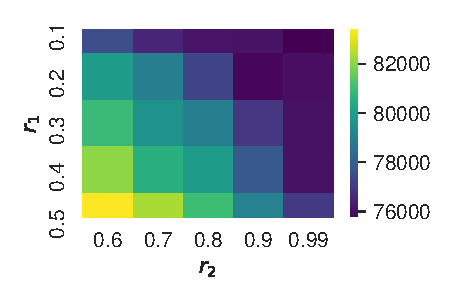
\includegraphics[width=0.24\textwidth]{../img/heatmap_N-t1d100_01}
  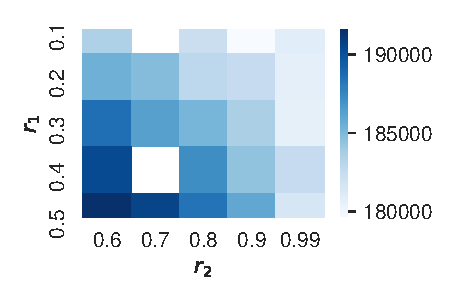
\includegraphics[width=0.24\textwidth]{../img/heatmap_N-t1d150_01}
  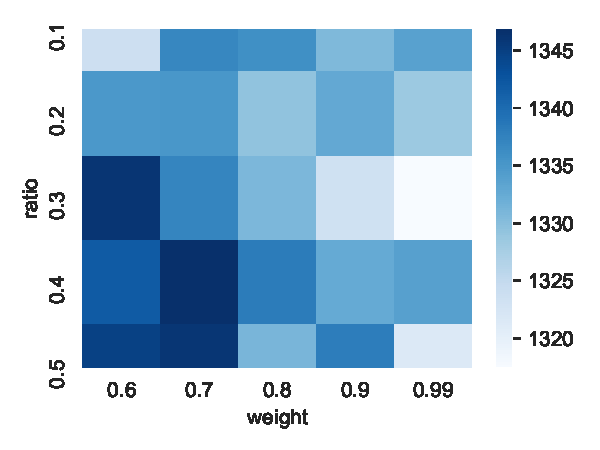
\includegraphics[width=0.24\textwidth]{../img/heatmap_rec05}
  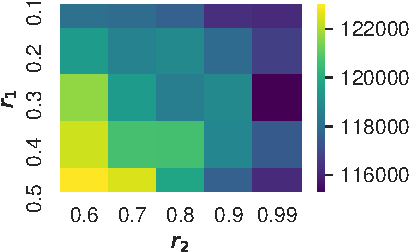
\includegraphics[width=0.24\textwidth]{../img/heatmap_kra32_dat}
    \caption{Mean fitness  (and standard deviation)  of each solution evaluated by each algorithm on LOP synthetic instances.\label{fig:heatmaps}}
\end{figure}

The plot shows that UMM is indeed very sensitive to the values of $r_1$ and
$r_2$, yet, low values of $r_1$ and high values of $r_2$ almost always produce
the best results, independently of the problem. Nevertheless, there are a few
cases where an interaction seems to occur and particular combinations perform
remarkably well.\MANUEL{why?}  In particular, we observe that the pattern on
the two left-most figures differs from the two right-most ones. While on the
left the fitness gets worse homogeneously from the top right corner to the
bottom left one, the pattern on the right is not as homogeneous, yet still
fitness gets worse with decreasing $r_2$.  We observe that this behavior is
related to the adequacy of UMM to the problem: the homogeneous behavior of
parameters $r_1$ and $r_2$ depends on the problem (not to the particular
instances) and the more homogeneous the behavior, the better performance of
UMM. We elaborate this argument in the following sections with detail.

Over all the instances \MANUEL{(which instances we tested? all synthetic?)} we
see that the configuration $r_1 =0.1$, $r_2=0.9$ has good
performance\MANUEL{how do you define this? The best mean?}. From this
preliminary experiment, it is not obvious how the best settings are related to
problem features, such as permutation length ($n$). On the other hand, given
the sharp transitions in the plots, it is clear that further fine-tuning may
improve performance and uncover further patterns.  Although automatic parameter
tuning may likely provide even more fine-tuned settings, our goal here is to
understand how UMM performs in comparison to an existing Bayesian method (CEGO)
and automatically tuning the parameters of CEGO is not computationally
feasible.  For consistency, in the following sections, we run UMM with this
parameter configuration. Moreover, we recommend this configuration as the
current default of UMM.

\subsection{Analysis of UMM and CEGO}

To better understand the behaviour of the algorithms, we record the fitness of
the solution evaluated at each step of each run and we average those values
over 10 runs with different random seeds on the same problem instance.  As an example, each line in Fig.~\ref{fig:lop_synth} 
shows the mean fitness of the solutions evaluated by either UMM or CEGO on one synthetic LOP
instance. The shaded area shows one standard deviation around the
mean. Ideally, each new evaluation will monotonically improve in fitness, since each solution evaluated helps to refine the model and leads to a
better solution being evaluated in the next step.  However, it is often the case that  \EKHINE{yo diría solo que lo esperable es que baje monotonically, sin entrar a valorar un ejemplo concreto}\MANUEL{Así está mejor? Quiero llamar la atención porque normalmente se muestra la evolución de la mejor solución encontrada pero nosotros estamos mostrando el fitness de cada solución evaluada}
% the fitness of the solutions does not improve monotonically and
new solutions
are often worse than their predecessors. Nevertheless, in this example, there
is a clear overall improvement as more evaluations are performed. The minimum
values achieved in the plot up to a particular number of function evaluations
gives an estimation of the mean fitness of the best-so-far solution up to that
point in the run. The algorithms do not return the final solution shown but
rather the best one (minimum fitness) of each run.


%: LOP syntéticas, todas en una gráfica. 
\begin{figure}[tb]
  \centering%
  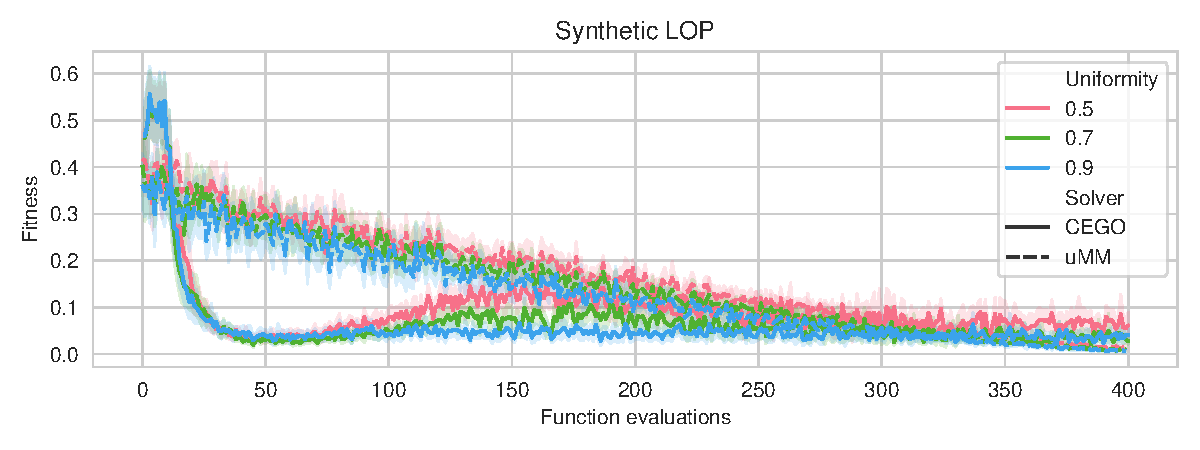
\includegraphics[width=\textwidth]{../img/synthetic_LOP_combined}
  \caption{Mean fitness  (and standard deviation)  of each solution evaluated by each algorithm on LOP synthetic instances.\label{fig:lop_synth}}
\end{figure}

When we compare the behaviour of CEGO and UMM on synthetic LOP instances
(Fig.~\ref{fig:lop_synth}), we observe a clear pattern independently of the
uniformity of the instances. In particular, CEGO starts with a random sampling
of X solutions, with are quite poor as expected, followed by building and
updating the Kriging model based new evaluations, which leads to an impressive
improvement in less than 50 evaluations. However, progress is more or less
halted at this point and the model seems to have trouble generating better
solutions. Lower uniformity values (e.g., $\mu=5$) show worsening evaluations
despite the increase in solutions used to build the model. In summary, the
Kriging model clearly helps CEGO to quickly identify good solutions in very few
evaluations. However, for some reason, CEGO is not able to further improve
those solutions given more data. This may due to the model not being able to
produce accurate predictions or the underlying optimizer not being able to find
improved solutions using the model.\MANUEL{perhaps we should measure the
  prediction error and see if it grows or decreases. That would answer this
  question.}


On the other hand, UMM converges much more slowly than CEGO, only reaching the
same fitness values around evaluation 250. Yet, UMM is able to keep the rate of
improvement and completely overtake CEGO around evaluation 350. As in the case
of CEGO, lower uniformity values lead to worse performance, although the
difference is much smaller for UMM than it was for CEGO.\MANUEL{If there is anything else we can say here, please go ahead and say it}


\newcommand{\supplement}{\citep{Supplementary}}


%: LOP reales: he puesto 3 de diferentes tamanos. Me ha parecido interesante que, a pesar de que CEGO parece que va mejor, esta diferencia se va reduciendo segun se aumenta el tamano del problema (que se puede ver en el nombre del problema y en el títutlo de la gráfica)
\begin{figure}[tbp]
  \centering%
  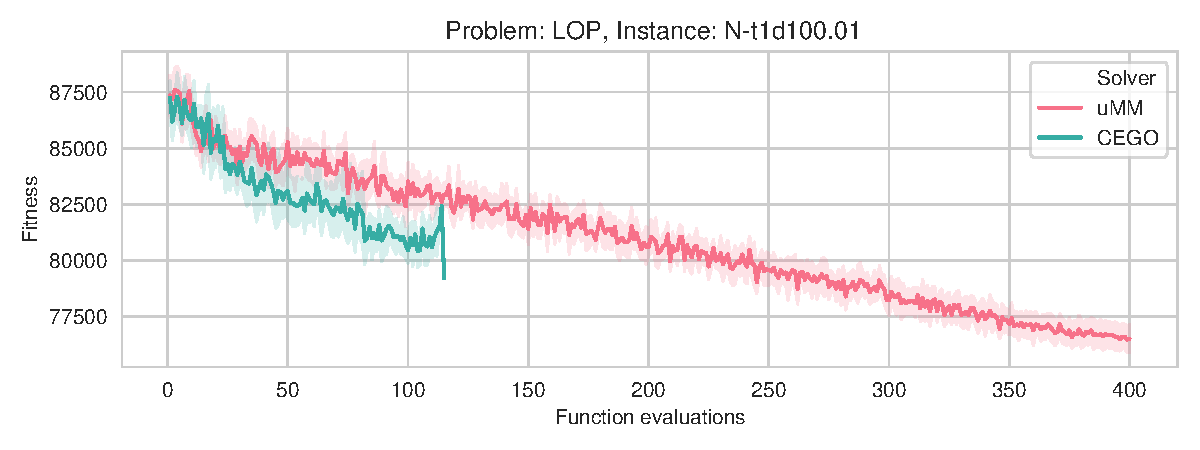
\includegraphics[width=\textwidth]{../img/fitness_real_lop_RandA1_N-t1d100_01}\\
  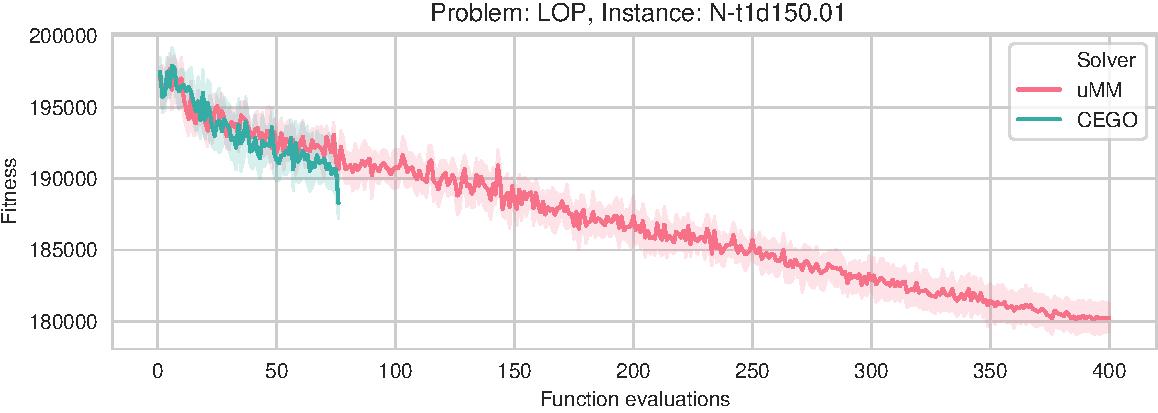
\includegraphics[width=\textwidth]{../img/fitness_real_lop_RandA1_N-t1d150_01}\\
  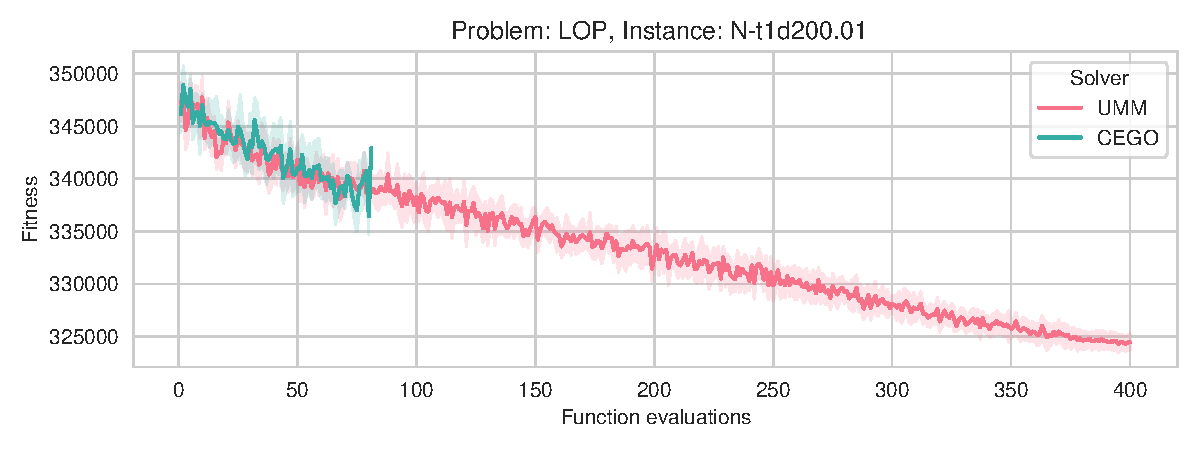
\includegraphics[width=\textwidth]{../img/fitness_real_lop_RandA1_N-t1d200_01}\\
    \caption{Mean fitness  (and standard deviation)  of each solution evaluated by each algorithm on three instances from LOPLIB.\label{fig:loplib}}
  \end{figure}


Results are quite different on the 
%The fast initial convergence of CEGO for synthetic LOP instances does not seem
%to translate to the
instances available in LOPLIB~\citep{}. We show in
Fig.~\ref{fig:loplib} three examples with different permutation size, however,
the results are consistent for other LOPLIB instances (complete results
available as supplementary material \supplement). Due to extremely long
runtimes of CEGO and constraints in our computing system, we set a maximum
wall-clock time of 3 days for each run of CEGO. On these instances, the
behaviour of CEGO and UMM is much more similar (at least up to the termination
point of CEGO). It appears that our synthetic LOP instances have a fitness
landscape that is very amenable to CEGO's Kriging model, whereas the LOPLIB
instances do not present such landscape. Comparing CEGO and UMM results, the
differences get smaller, in favour of UMM, with larger instance size. Our
conjecture is that building an accurate Bayesian model and searching for good
solutions on it becomes harder for larger fitness landscapes.
\EKHINE{Parece que el paper va del CEGO en vez del UMM :p. Yo diría que tanto UMM como CEGO encuentran soluciones que mejoran según avanzan, pero con diferencias de comportamiento: (1) las los optimos de UMM son '3 veces mejor', y esto yo creo que es importante, aunque en gran parte se debe a que (2) UMM hace 400 ejecuciones en 3, 6 y 11 horas y CEGO entre 50 y 130 en 5 dias (3) cego empeora segun n aumenta (y n=200 tampoco es enorme)}
\MANUEL{Eso es porque puedo interpretar los resultados de CEGO mejor que los de UMM. Si crees que hay alguna interpretación o conjetura sobre UMM que podemos mencionar aquí, sería bueno mencionarla.}
\MANUEL{Prefiero dejar el comentario sobre las mejores soluciones encontradas y el tiempo requerido para cuando hable de la tabla, así se puede ver todo junto}

In the case of the PFSP, none of the algorithms are able to achieve a progress
better than a random search would, as illustrated by the results
(Fig.~\ref{fig:rec05}) obtained on \texttt{rec05}, which is the smallest PFSP
instance considered here. The lack of any apparent convergence suggests that
the models (both Bayesian and probabilistic) are not learning anything about
the fitness landscape. Results for larger PFSP corroborate this conclusions
(\supplement). Although previous studies~\citep{ZaeStoBar2014:ppsn} concluded
that other distance measures are more suited than Kendall's-$\tau$ distance for
the PFSP, the reported fitness differences between various distance metrics are
small, hence, we conjecture that the same behaviour will be observed with other
distance metrics.
  

\begin{figure}[tb]
  \centering%
  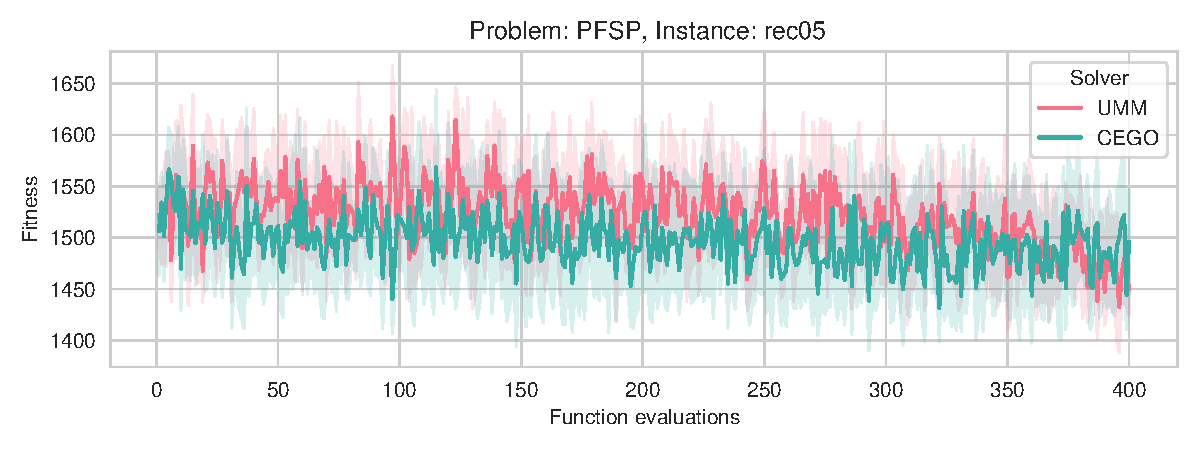
\includegraphics[width=\textwidth]{../img/fitness_real_pfsp_rec05_txt}
  \caption{Mean fitness  (and standard deviation)  of each solution evaluated by each algorithm on the PFSP instance \texttt{rec05}.\label{fig:rec05}}
\end{figure}

The situation is very similar for the QAP, where both algorithms show the same
behaviour as in the PFSP for all instances tested, except for
\texttt{kra32}. As shown in Fig~\ref{fig:kra32}, in this instance both
algorithms are able to improve over the number of evaluations, although not
with ease. As in the synthetic LOP instances, we again observe that CEGO does
improve faster than UMM initially, yet, around evaluation 250, it appears to
get stuck and around evaluation 300, UMM overtakes it. We believe the reason is
the same as before, that is, the model is not able to adequately reflect the
ruggedness of the actual landscape and, hence, the best solutions found by the
GA searching the model are not improved solutions for the actual problem. Interestingly, \texttt{kra32} is rectangular
whereas \texttt{tho32} contains rectangular distances and \texttt{nug12} and \texttt{nug30} contain Manhattan distances of rectangular grids.\MANUEL{so they all have the same distance type!!! What is the difference then? Ask Thomas?}

\begin{figure}[tp]
  \centering%
  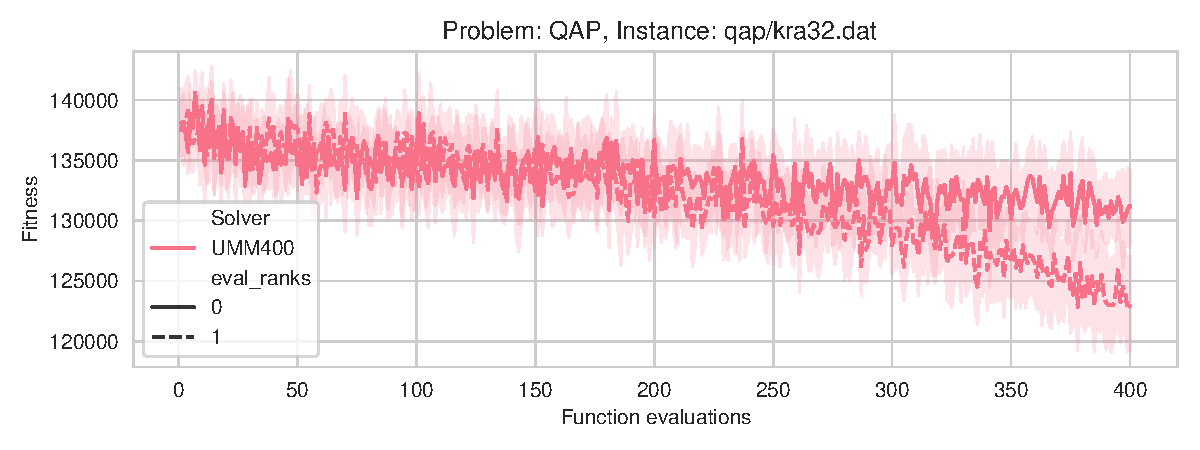
\includegraphics[width=\textwidth]{../img/fitness_real_qap_kra32_dat}
    \caption{Mean fitness  (and standard deviation)  of each solution evaluated by each algorithm on the QAP instance \texttt{kra32}.\label{fig:kra32}}
\end{figure}

Table~\ref{tab:results} shows overall results over all instances evaluated (excluding the synthetic LOP instances). In particular, the mean fitness (and standard deviation) of the best solution found at the end of each run,
In terms of best fitness achieved on each run, and taking into account the
random behaviour observed in some instances and discussed above,



\newcommand{\mcolc}[2]{\multicolumn{#1}{c}{\bf #2}}
\begin{table}[tb]
 \caption{Mean fitness (and standard deviation) of the best solution found at the end of each run, over 10 independent runs for each problem instance. The 95\% confidence interval corresponds to the two independent samples t-test on the mean of the difference between the fitness of UMM minus the one of CEGO. Mean runtime is measured in hours. If a run went over 72 hours, of  CEGO was not able to reach 400 function evaluations (FEs) in 72 hours, it was terminated earlier. This was the case for all LOP instances shown.\manuel{}{Don't we have results for rec31?}\label{tab:results}}
 \resizebox{\textwidth}{!}{%
\begin{tabular}{r@{\hskip -2ex}*{5}{r}rl@{\hskip -2ex}*{3}{r}}
 \toprule
            &                  & \mcolc{4}{Mean fitness (sd)} & \mcolc{2}{\multirow[b]{2.45}{*}{\shortstack{95\% CI of the\\mean difference}}} & \bf \multirow[b]{2.45}{*}{\shortstack[r]{Mean FE\\CEGO}} & \mcolc{2}{Mean runtime} \\\cmidrule(lr){3-6}\cmidrule(lr){10-11}
\bf Problem & \bf     Instance & \mcolc{2}{CEGO} & \mcolc{2}{UMM}   &                         &            & \bf & \bf CEGO       & \bf UMM                       \\\midrule
    LOP     & N-t1d100.01      & 78696.6                 & (811.4)    & 76119.6   & (915.4)                & $[$1763.5,    & 3390.5$]$     & 111.8& 72.5 & 3.2  \\
     & N-t1d100.02      & 79686.5                 & (367.9)    & 76827.7   & (891.0)                & $[$2194.5,    & 3523.1$]$     & 110.7& 72.9 & 3.2  \\
     & N-t1d150.01      & 187605.5                & (1906.9)   & 179508.3  & (1647.9)               & $[$6420.3,    & 9774.1$]$     & 73.9 & 72.7 & 6.5  \\
     & N-t1d150.02      & 184320.9                & (973.5)    & 177592.8  & (1196.2)               & $[$5700.5,    & 7755.7$]$     & 74.1 & 73.2 & 6.5  \\
     & N-t1d200.01      & 335391.1                & (2289.0)   & 323513.6  & (1371.2)               & $[$10076.1,   & 13678.9$]$    & 55.6 & 73.2 & 10.7 \\
     & N-t1d200.02      & 333149.5                & (2497.2)   & 319675.8  & (2242.6)               & $[$11242.0,   & 15705.4$]$    & 56.5 & 73.7 & 10.6 \\
     & N-t2d150.01      & 24682.7                 & (976.6)    & 15297.7   & (563.5)                & $[$8622.2,    & 10147.8$]$    & 74.6 & 72.9 & 7.0  \\
     & N-t2d150.02      & 24250.8                 & (1354.9)   & 14724.9   & (667.5)                & $[$8495.1,    & 10556.7$]$    & 74.8 & 72.8 & 7.1  \\
     & N-t2d200.01      & 57098.6                 & (4452.8)   & 33465.2   & (2001.0)               & $[$20284.5,   & 26982.3$]$    & 56.3 & 73.3 & 11.2 \\
     & N-t2d200.02      & 54895.6                 & (4589.7)   & 35901.8   & (2077.5)               & $[$15539.1,   & 22448.5$]$    & 55.6 & 73.5 & 11.2 \\
     & N-p50-01         & 21431.2                 & (299.5)    & 21027.6   & (711.8)                & $[$-128.1,    & 935.3$]$      & 219.9& 72.3 & 0.9  \\
     & N-p50-02         & 22021.1                 & (275.6)    & 21613.6   & (596.4)                & $[$-42.5,     & 857.5$]$      & 217.3& 72.3 & 0.9  \\
     & N-atp111         & 693.1                   & (10.3)     & 594.0     & (15.4)                 & $[$86.7,      & 111.5$]$      & 98.7 & 72.5 & 4.1  \\
     & N-atp134         & 880.5                   & (18.6)     & 756.3     & (21.3)                 & $[$105.4,     & 143.0$]$      & 83.0 & 72.8 & 5.7  \\
     & N-be75eec\_150   & 1666193.1               & (72310.8)  & 1415208.5 & (58593.5)              & $[$188960.6,  & 313008.6$]$   & 74.0 & 72.9 & 6.9  \\
     & N-be75eec\_250   & 5214413.0               & (166701.4) & 4431271.0 & (109756.7)             & $[$649040.8,  & 917243.2$]$   & 44.9 & 73.7 & 15.5 \\
     & N-be75np\_150    & 3742444.0               & (88500.2)  & 3204878.3 & (80704.1)              & $[$457944.2,  & 617187.2$]$   & 74.2 & 72.9 & 6.9  \\
     & N-be75np\_250    & 10887427.8              & (159642.5) & 9544754.9 & (260523.9)             & $[$1136635.8, & 1548710.0$]$  & 45.3 & 74.0 & 15.5 \\\midrule
   PFSP     & rec05        & 1317.9                  & (25.1)     & 1330.7    & (17.9)                 & $[$-33.4,     & 7.8$]$        & 400.0& 38.9 & 0.1  \\
       & rec13        & 2128.2                  & (25.0)     & 2158.7    & (29.5)                 & $[$-56.2,     & -4.8$]$       & 400.0& 38.9 & 0.1  \\
       & rec19        & 2398.6                  & (19.8)     & 2405.1    & (12.6)                 & $[$-22.3,     & 9.3$]$        & 400.0& 82.1 & 0.3  \\\midrule
    QAP     & kra32        & 115907.0                & (4663.4)   & 116320.0  & (4673.5)               & $[$-4799.3,   & 3973.3$]$     & 400.0& 95.8 & 0.3  \\
        & nug12        & 624.2                   & (26.3)     & 660.4     & (17.3)                 & $[$-57.3,     & -15.1$]$      & 400.0& 14.8 & 0.0  \\
        & nug30        & 7486.8                  & (40.4)     & 7474.0    & (83.9)                 & $[$-50.8,     & 76.4$]$       & 400.0& 84.3 & 0.3  \\
        & tho30        & 192416.0                & (2584.2)   & 191482.0  & (4419.7)               & $[$-2527.0,   & 4395.0$]$     & 400.0& 85.1 & 0.3  \\
\bottomrule
\end{tabular}}
\end{table}




\section{Conclusions}

In this paper, we have introduced UMM, a population-based probabilistic
algorithm based on an unbalanced Mallows model. The algorithm is designed for
black-box combinatorial problems on permutation landscapes and when the budget
of fitness evaluations is severely limited (up to $1000$ or less).  UMM is
specially well-suited for budget-limited scenarios that are still
time-sensitive, e.g., when the overhead incurred by the optimizer should be no
more than a few minutes added to each fitness evaluation. As shown by our
results, a Bayesian optimizer such as CEGO may sometimes require more than hour
per fitness evaluation. The time required to train the surrogate-model of CEGO
also sharply increases with permutation length, hence, UMM would be a
computationally feasible alternative for relatively large problem sizes.

Although we were inspired by previous work on ACO for expensive black-box
combinatorial problems~\citep{PerLopStu2015si}, UMM is, to the best of our
knowledge, the first EDA specifically designed for such problems that is able
to obtain competitive results when compared with Bayesian optimizers. The
results presented here show that, despite the intrinsic difficulty of this scenario, there are still significant advances yet to be made. Thus, we hope
that this paper will motivate further research. % on such problems.

A somewhat surprising result was that the behavior of UMM (and the same for
CEGO) on the PFSP is close to random. This result may be due to the distance
metric used, but further analysis is needed to corroborate this
conjecture. Here, we have focused on Kendall's $\tau$ distance, however, it is
possible to extend UMM to other distance metrics, which will allow us to
dynamically select among various distance metrics for an unknown black-box
permutation landscape~\citep{ZaeStoBar2014:ppsn}. Also, as shown by our
experiments, the behavior of the parameters ($r_1$ and $r_2$) of UMM is not
always obvious, thus a more detailed analysis would be needed to provide either
generally good static values or an online adaptation approach. Finally, we have
used here three very different combinatorial problems (LOP, PFSP and QAP) as
black-box benchmarks. However, an even more diverse range of problems would be
needed to understand the behavior of UMM on real-world black-box combinatorial
landscapes.

% Bayesian optimization methods using a global GP model, such as CEGO, are known
% to have trouble optimizing locally \citep{EriPeaGar2019scalable}. Our
% intuition is that this problem becomes worse in rugged combinatorial
% landscapes, where small steps may produce drastic changes.

% Open questions:
% \begin{itemize}
% \item How difficult is to extend UMM to other distance metrics?
% \item Can we plot the posterior probability of the optimal solution?
% \end{itemize}

%% MANUEL: Blind, so no acknowledgments yet.
\begin{smaller}
\paragraph*{Acknowledgements.}
% M.\@ L\'opez-Ib\'a\~nez is a ``Beatriz Galindo'' Senior Distinguished Researcher (BEAGAL 18/00053) funded by the Ministry of Science and Innovation of the Spanish Government.
%
Thanks to Hao Wang (Leiden University) for pointing us to the arguments of
\citet{EriPeaGar2019scalable}.
\end{smaller}



\renewcommand{\doi}[1]{doi:\hspace{.16667em plus .08333em}\discretionary{}{}{}\href{https://doi.org/#1}{\urlstyle{rm}\nolinkurl{#1}}}
\bibliographystyle{splncs04nat}
\bibliography{optbib/abbrev,optbib/authors,optbib/journals,optbib/biblio,optbib/crossref,./mendeley}

\end{document}

%%% Local Variables:
%%% mode: latex
%%% TeX-master: t
%%% End:
